% ============================================================
%  Introduction — H&E to Sirius Red Virtual Staining Paper
%  Compile with: pdflatex + bibtex (or biblatex/biber)
%  NOTE: [TBC] markers denote citations needing author verification
% ============================================================
\section{Introduction}

Histopathology in most cases relies on a panel of stains.
Hematoxylin and eosin~(H\&E), the most widely available routine stain, reveals overall
tissue architecture, while specialised histochemical stains highlight specific tissue
components such as collagen fibres, and immunohistochemical stains visualise
particular proteins via antibody binding to infer cell types or functional states such
as proliferation or necrosis~\cite{lefkowitch2006special, krishna2013role}.
In clinical and preclinical practice, however, each additional stain requires a separate
tissue section. This consumes limited biopsy material~\cite{rivenson2020emerging, dehaan2021deep},
extends laboratory processing time~\cite{dehaan2021deep}, raises per-case reagent and
labour cost (substantially so for antibody-based panels), and introduces spatial
misalignment between stains because tissue deforms during sectioning and
mounting~\cite{gatenbee2023virtual, chen2022mvfstain}.
These costs grow with each additional stain: a full tissue characterisation panel may
require four or more serial sections from a single
biopsy~\cite{clark2017immunohistochemistry}, and because a biopsy yields only a
limited number of usable sections, every extra stain trades against either reserve
material for downstream molecular assays or the breadth of complementary stains that
can be examined on the same specimen.

Liver pathology is a particularly acute case.
Chronic liver disease is staged primarily by the degree of fibrosis, the progressive
deposition of collagen in the extracellular matrix, which is the principal predictor of
long-term outcome.
While fibrosis can be qualitatively appreciated on H\&E, Sirius Red~(SR) provides the
standard \emph{quantitative} readout: SR binds collagen with high specificity and is the
histochemical stain of reference for measuring fibrosis as the collagen proportionate
area~(CPA), correlating more strongly with serum fibrosis biomarkers than the widely
used Masson's trichrome stain~\cite{huang2013sirius}.
Inferring SR directly from a routinely acquired H\&E section would therefore make a
clinically meaningful fibrosis readout available wherever H\&E is, without consuming
additional tissue or laboratory resources.

Virtual staining offers an attractive solution: it uses deep learning to predict a
target stain directly from an existing H\&E image
(Figure~\ref{fig:pipeline_overview}), and additionally enables retrospective analysis of
existing H\&E archives without acquiring new
sections~\cite{rivenson2020emerging, latonen2024virtual}.
Supervised approaches, however, require pixel-aligned image pairs from adjacent tissue sections,
which is impractical at scale and introduces bias from tissue
deformation~\cite{aatresh2024virtual}.
\textit{Unsupervised} methods, which learn from unpaired image collections, are better
suited to this setting. However, no prior work has systematically compared them for
H\&E~$\to$~SR translation in liver tissue; existing comparisons focus almost entirely on
H\&E~$\to$~IHC or on non-liver
tissue~\cite{visgab2025, adib2024dual, klockner2025he}.
The existing benchmarks fix a single model scale and data budget~\cite{visgab2025, klockner2025he},
leaving open how model capacity and training data jointly affect translation quality, an
important question because liver biopsy cohorts vary widely in size across clinical centres.

\begin{figure*}[t!]
  \centering
  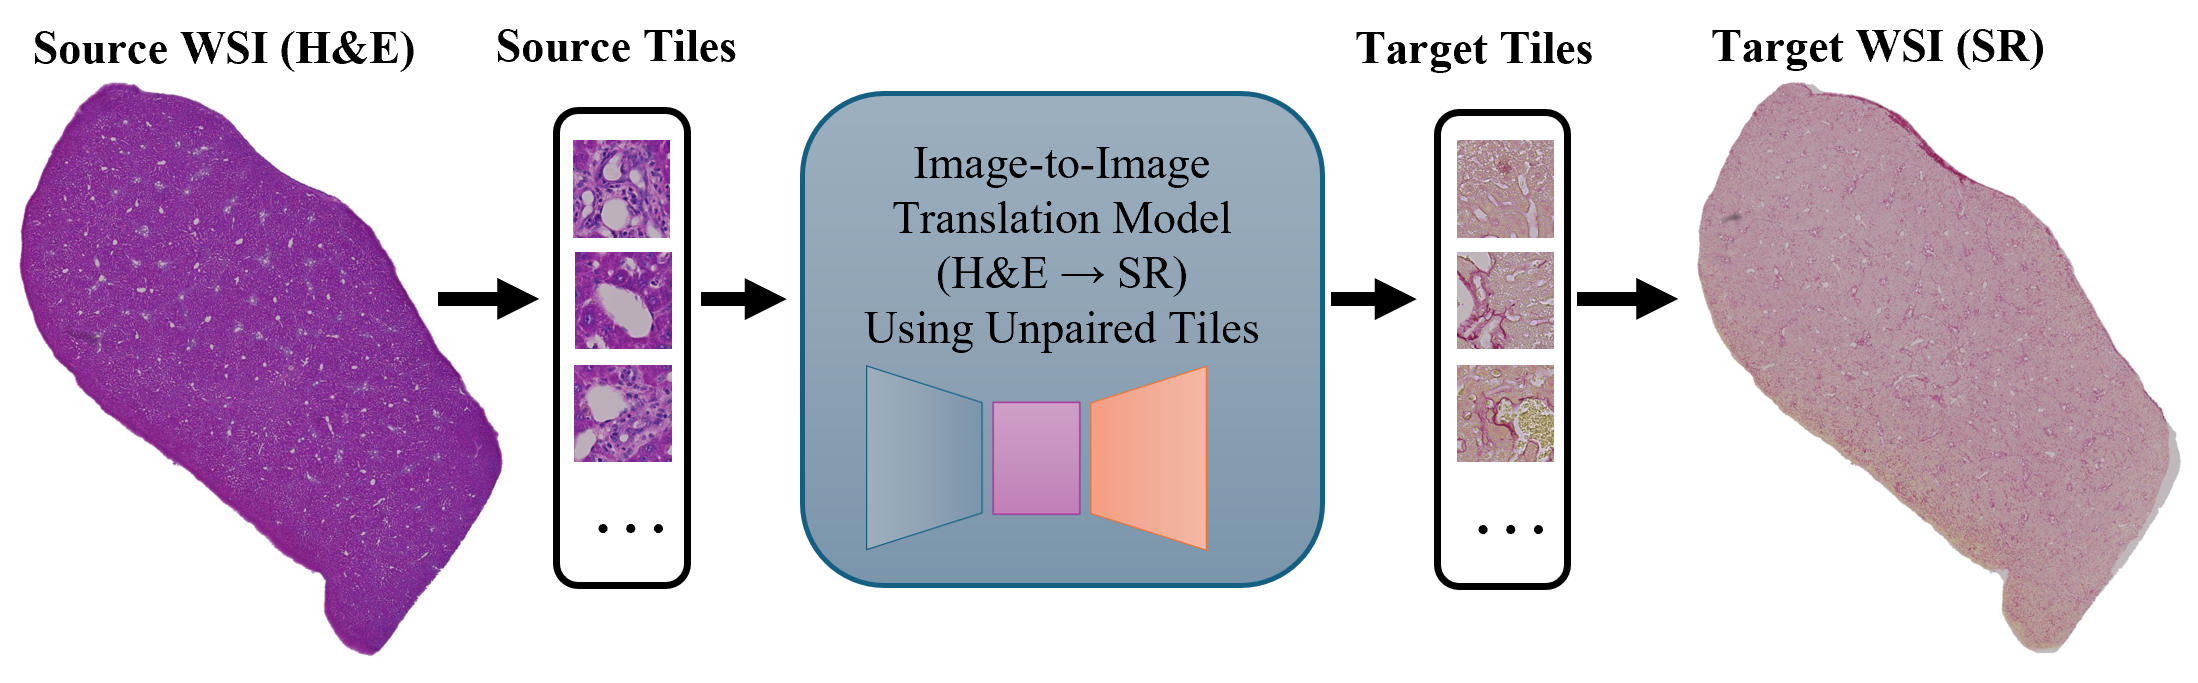
\includegraphics[width=0.90\linewidth]{images/translation.png}
  \caption{%
    Overview of the virtual H\&E~$\to$~SR staining pipeline studied in this work.
    A whole-slide image~(WSI) acquired with H\&E staining is decomposed into
    $256{\times}256$\,pixel tiles, which are passed through an unpaired
    image-to-image~(I2I) translation model to produce virtual Sirius Red tiles.
    The translated tiles are reassembled into a virtual SR WSI, from which
    collagen proportionate area~(CPA) can be quantified without requiring a
    second, physical SR-stained section from the same tissue block.
  }
  \label{fig:pipeline_overview}
\end{figure*}

Beyond translation quality, we also need a signal of when a virtual SR output can be
trusted. Task-specific evaluation can verify aggregate translation quality at the WSI
level (Section~\ref{sec:metrics}), but in unpaired settings no ground-truth SR is available for any given
H\&E tile, so individual tile outputs cannot be checked against truth even though
clinical decisions may hinge on local features within a single tile.
Training ensembles of independently seeded models and comparing their outputs reveals where
they converge on the same answer and where they do not on tile level: disagreement flags inputs for
which the unsupervised objective does not pin down a unique translation, providing an
indicator of epistemic uncertainty that complements task-specific evaluation.

Consequently, we present three main results that advance unsupervised stain
translation toward more reliable and uncertainty-aware evaluation.

First, to map where translation quality actually lies in the design space of model
capacity and training-data budget, we conduct a full-factorial scaling study of six
unsupervised I2I architectures spanning GAN-based and diffusion-based families
(CycleGAN~\cite{zhu2017unpaired}, UNIT~\cite{liu2017unsupervised},
MUNIT~\cite{huang2018multimodal}, DCLGAN~\cite{han2021dual},
UVCGAN~\cite{torbunov2022uvcgan}, and CycleDiffusion~\cite{wu2022cyclediffusion}) at
three generator capacities (${\sim}10$, ${\sim}50$, ${\sim}100$~million parameters) and
three data fractions (25\%, 50\%, 100\%). Each of the 54 configurations is evaluated
using a task-specific CPA mean absolute error~(CPA~MAE), computed by applying a frozen
collagen segmentation model to real and virtual SR images, alongside three perceptual metrics: FID (distributional
realism), LPIPS (perceptual similarity), and patch-SSIM (local structural similarity).
Reporting all four metrics jointly exposes where perceptual rankings agree with
task-level accuracy and where they diverge.

Building on this study, to quantify where these models are committed to a single
answer and where they are not, we train deep ensembles of independently seeded
models for the best configuration per family, producing spatially resolved uncertainty
maps. We provide the first systematic comparison of epistemic uncertainty across unsupervised
stain-to-stain architectures.

%Finally, to enable independent benchmarking and reproducible evaluation by the
%community, we release the dataset of 35 paired H\&E and Sirius Red specimens
%(70 WSIs) from a mouse bile-duct ligation~(BDL)
%experiment~\cite{ghallab2025asbt}, the first open resource for unsupervised
%H\&E~$\to$~SR translation in mouse liver tissue.
% ============================================================
%  Bibliography entries specific to this section
%  (merge with references.bib; shared entries already in related_work.tex)
% ============================================================
%
% @article{Bataller2005,
%   author  = {Bataller, Ramon and Brenner, David A.},
%   title   = {Liver fibrosis},
%   journal = {Journal of Clinical Investigation},
%   volume  = {115},
%   number  = {2},
%   pages   = {209--218},
%   year    = {2005},
%   doi     = {10.1172/JCI24282}
% }
%
% @article{huang2013sirius,
%   author  = {Huang, Yi and de Boer, Wilhelmina B. and Adams, Leon A. and MacQuillan, Gerry and Bulsara, Max K. and Jeffrey, Gary P.},
%   title   = {Image analysis of liver collagen using sirius red is more accurate and correlates better with serum fibrosis markers than trichrome},
%   journal = {Liver International},
%   volume  = {33},
%   number  = {8},
%   pages   = {1249--1256},
%   year    = {2013},
%   doi     = {10.1111/liv.12184}
% }
%
% (All other entries shared with related_work.tex:
%  rivenson2020emerging, latonen2024virtual, kieffer2020largescale, li2023unpaired,
%  aatresh2024virtual, zhu2017unpaired, liu2017unsupervised, huang2018multimodal,
%  han2021dual, torbunov2022uvcgan, wu2022cyclediffusion, visgab2025, adib2024dual,
%  gal2016dropout, lakshminarayanan2017simple, uncertainty_informed_hist2022,
%  liverfibrosis2025, ugac2021, trustworthy_i2i2025)